\chapter{Moléculas Fotónicas \label{cap:molecules}}

La técnica de escritura de guías de onda descrita en el Capítulo~\ref{cap:fs} está restringida por la forma alargada y elíptica del tren de pulsos láser que se enfoca, lo que limita los acoplamientos interorbitales posibles \citep{interorbital}. Una alternativa para aumentar los grados de libertad consiste en fabricar dos guías de onda suficientemente cercanas para hibridizar sus modos guiados, de manera análoga al principio físico que gobierna las moléculas. Por este motivo, en este capítulo se empleará el concepto de \textit{moléculas fotónicas} \citep{molecules}, aplicándolo al estudio experimental de una red fotónica que presenta una doble transición de fase topológica \citep{SPSSH}.

\section{Autoestados del acoplador fotónico para distancias de separación pequeñas}

Como se mencionó en la Sección~\ref{cap:CMT}, la teoría de modos acoplados (CMT) describe adecuadamente los sistemas fotónicos en estudio cuando la distancia entre guías de onda supera los $13\,\mu$m. Para separaciones menores, el sistema debe tratarse como una única macroguía. La expansión en modos normales (EME), presentada en la Sección~\ref{cap:eme}, proporciona una herramienta numérica válida para ambos regímenes. 

Mediante simulaciones de pares de guías de onda a diferentes distancias, se caracterizó el comportamiento de sus autoestados. La Figura~\ref{fig:molecule-coup} muestra que el autoestado antisimétrico ($+-$) solo existe para distancias mayores a $13\,\mu$m, ya que por debajo de este umbral se convierte en un modo de radiación ($k_z^{+-} < k_0 n_0$). En cambio, el autoestado simétrico ($++$) persiste y puede describirse como una única entidad, lo que en esta tesis se denominará \textit{modo S} de la molécula fotónica.

\begin{figure}[H]
	\centering
	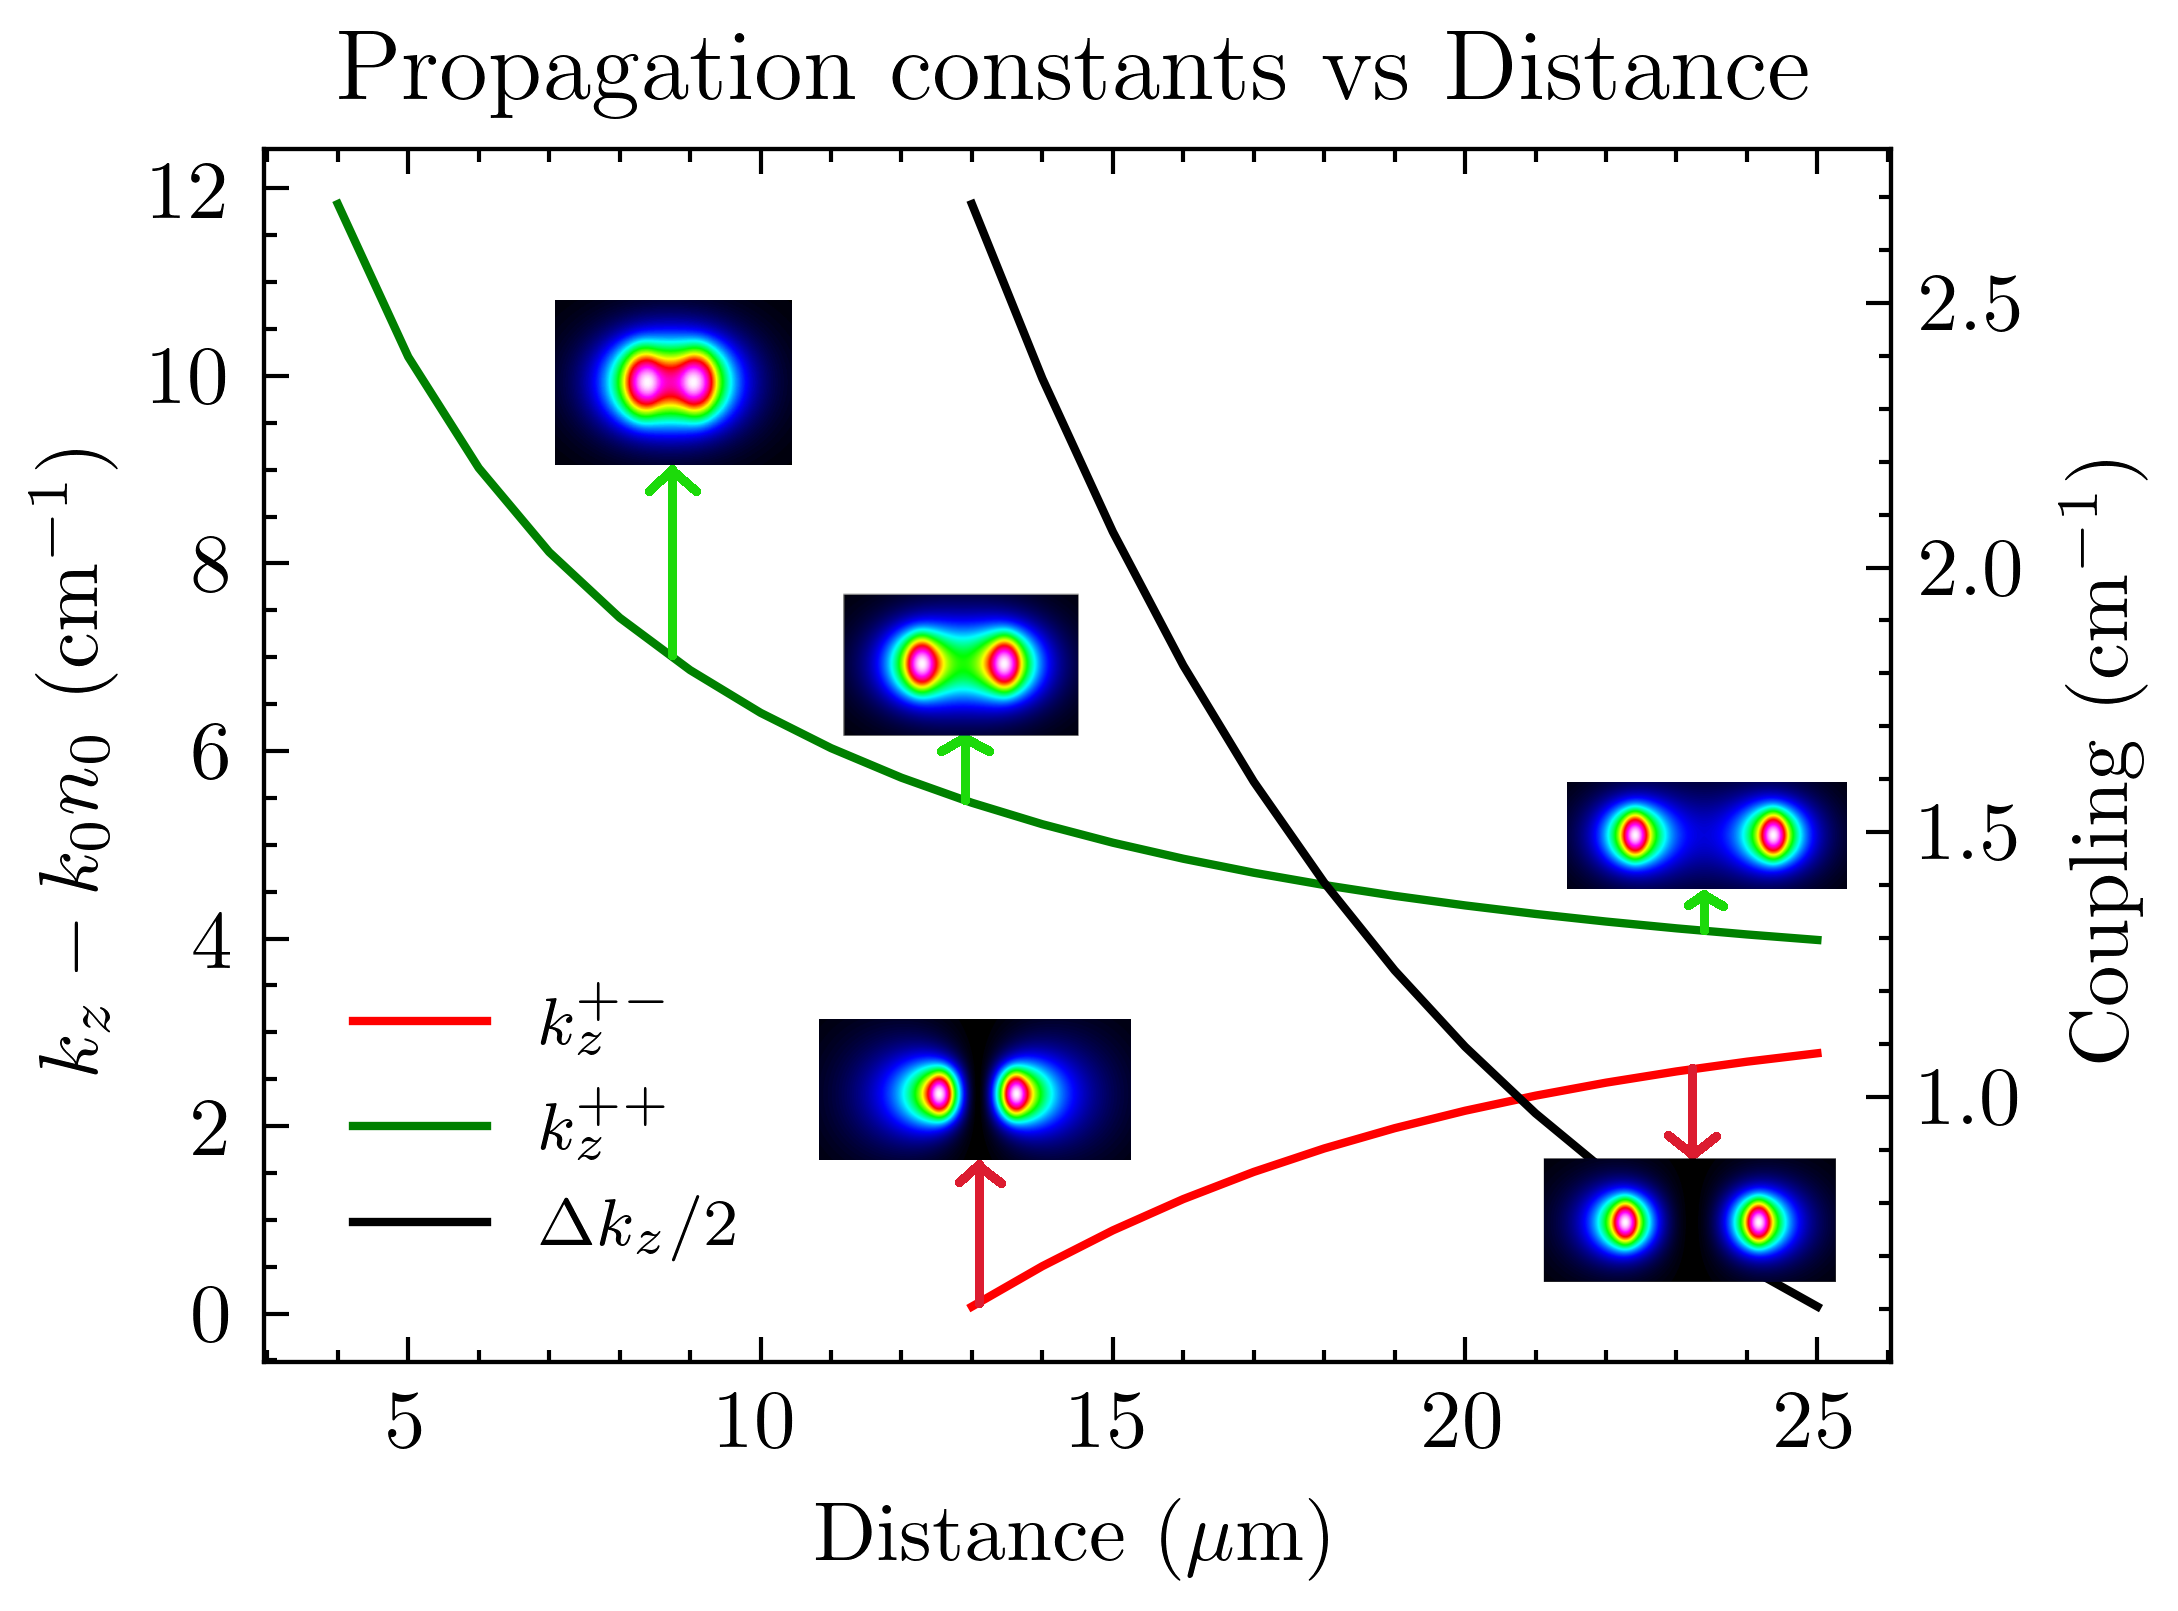
\includegraphics[width=0.46\linewidth]{codigo/dimol2/eigenvalues_vs_angle_1.png}
	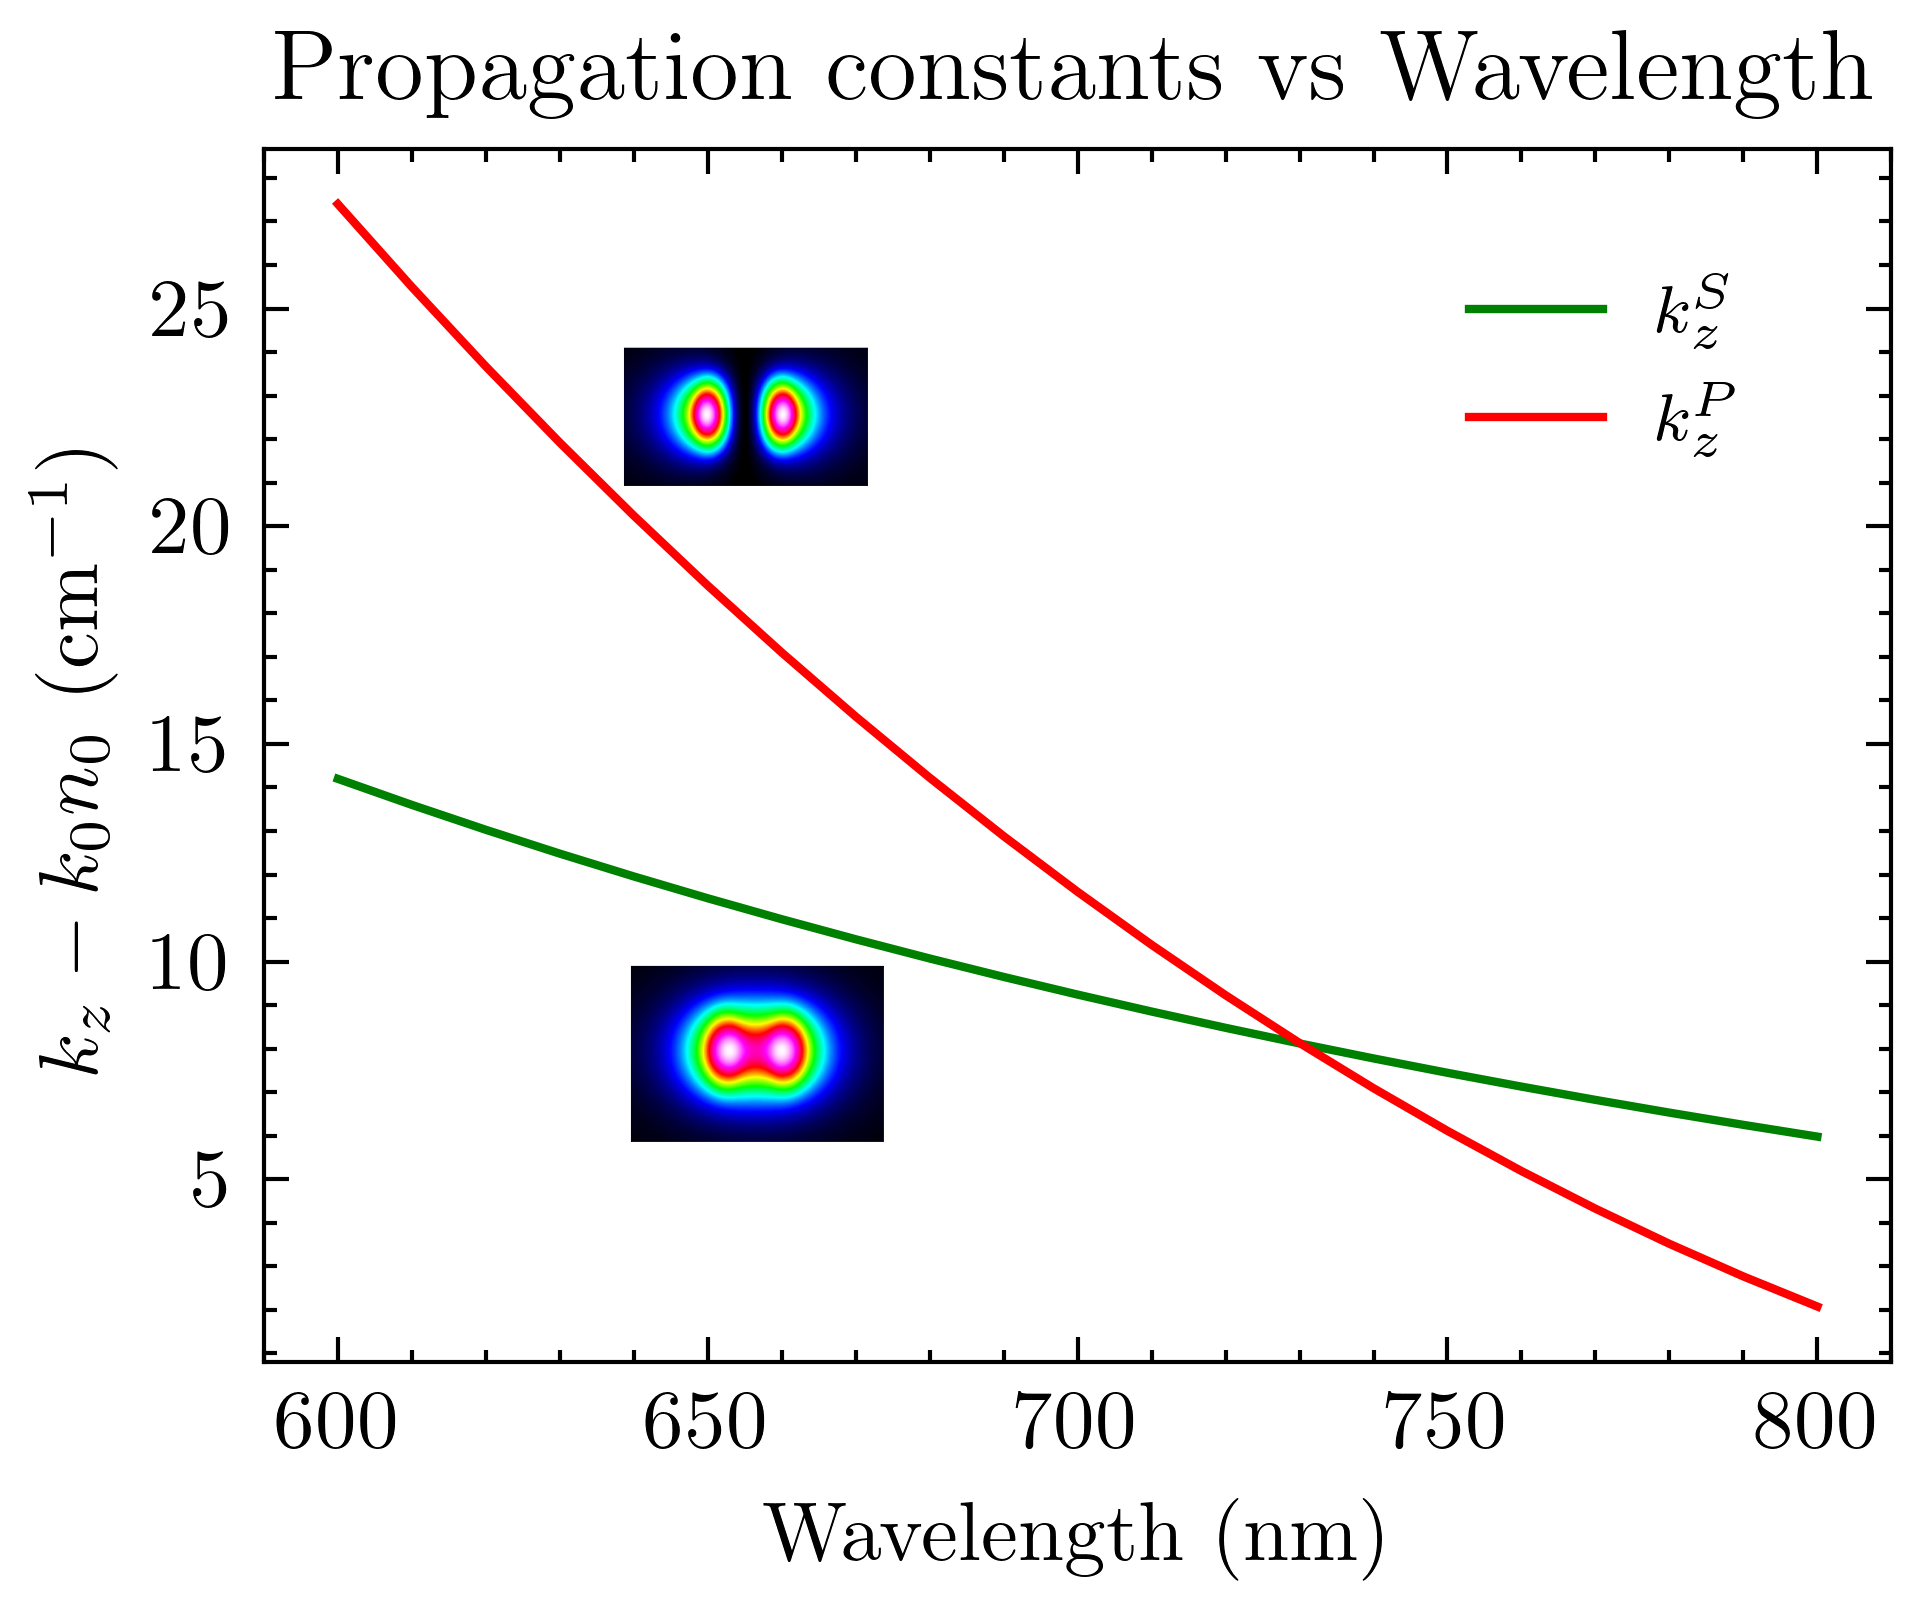
\includegraphics[width=0.40\linewidth]{codigo/dimol3/eigenvalues_vs_wavelength.png}
	\caption[Propagación y acoplamientos en moléculas fotónicas]{
		\textbf{Izquierda:} Constantes de propagación y acoplamientos en función de la distancia para modos fundamentales, calculados mediante EME. 
		\textbf{Derecha:} Constantes de propagación de modos $S$ y $P$ en función de la longitud de onda.
		\label{fig:molecule-coup}}
\end{figure}

Si bien las constantes de propagación de los modos $S$ y $P$ en una misma molécula presentan valores diferentes, estas pueden igualarse entre moléculas adyacentes mediante el ajuste del contraste de índice de refracción en las guías de onda \citep{interorbital}. Por ejemplo, la Figura~\ref{fig:molecule-coup} muestra que a $730$\,nm se igualan las constantes de propagación para $\Delta n_S = 5.200 \times 10^{-4}$ y $\Delta n_P = 10.423 \times 10^{-4}$.

\section{Moléculas Fotónicas en Red SP-SSH}

Para la implementación experimental (Sección~\ref{cap:fs}) de una red que presente acoplamiento SP \citep{interorbital, toporusos, SPSSH}, se utilizaron los modos $P$ horizontales de la sección anterior, obtenidos mediante moléculas fotónicas. Un preciso sintonizado de las constantes de propagación de los modos $S$ ($k_z^S$) y $P$ ($k_z^P$) permitió considerar un grado de libertad análogo al del espín del electrón (\textit{pseudoespín}). El Hamiltoniano $H$ de esta red \citep{SPSSH}, ilustrado en la Figura~\ref{fig:sp-ssh-model}, es el siguiente:
\begin{align*}
	H &= \sum_n \left[\frac{\delta\beta}{2} \left( p^*_{n, 1} p_{n, 1} - s^*_{n, 1} s_{n, 1} + p^*_{n, 2} p_{n, 2} - s^*_{n, 2} s_{n, 2} \right) + \varkappa_{ss, 2}s^*_{n, 2} s_{n, 1} - \varkappa_{pp, 2}p^*_{n, 2} p_{n, 1} \right. \\
	&+ \varkappa_{ss, 1} \left( s_{n-1, 2}^*s_{n, 1} + s_{n+1, 2}^*s_{n, 2} \right) - \varkappa_{pp, 1} \left( p_{n-1, 2}^*p_{n, 1} + p_{n+1, 2}^*p_{n, 2} \right) + \varkappa_{sp, 2} \left( s_{n, 2}^* p_{n, 1} - p_{n, 2}^* s_{n, 1} \right) \\
	&+ \left. \varkappa_{sp, 1} \left( s_{n-1, 2}^* p_{n, 1} - p_{n-1, 2}^* s_{n, 1} + s_{n+1, 1}^*p_{n, 2} - p_{n+1, 1}^* s_{n, 2} \right) \right] + \text{c.c.}
\end{align*}

\begin{figure}[H]
	\centering
	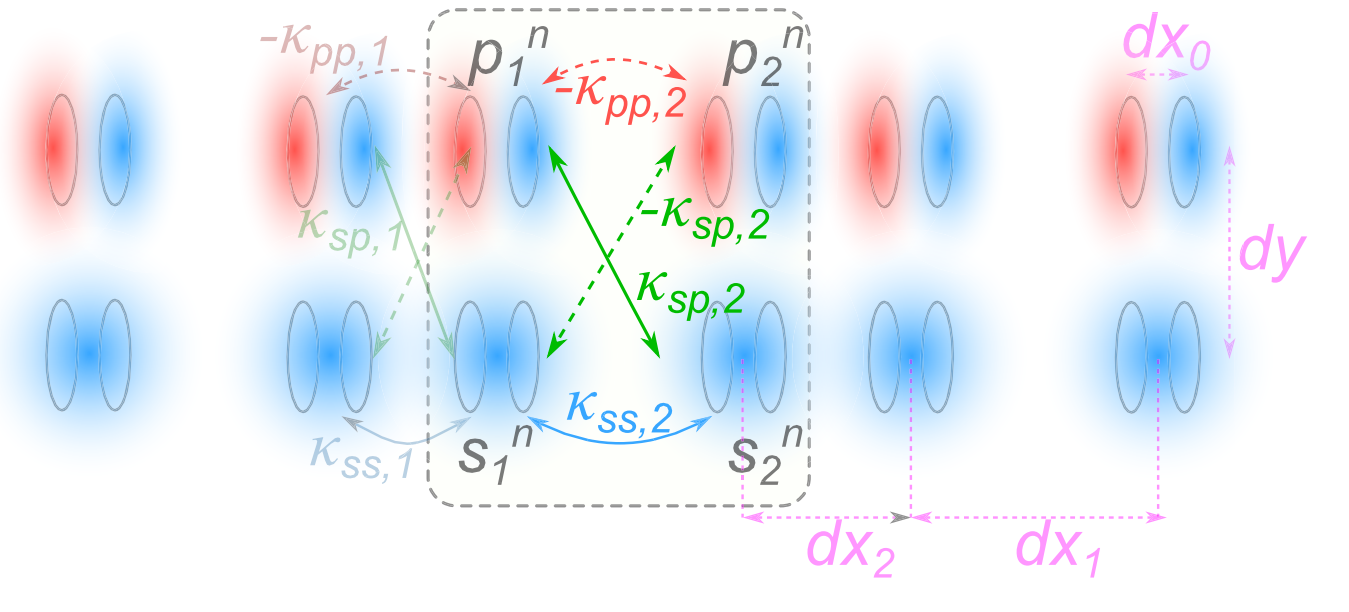
\includegraphics[width=0.8\linewidth]{media/ssh_sp_model}
	\caption{Esquema de la red SP-SSH y los acoplamientos considerados. \label{fig:sp-ssh-model}}
\end{figure}

Si se elige la base $\mathbf{v}^n = \left( s_1^n, p_1^n, s_2^n, p_2^n \right)^T$, el Hamiltoniano de Bloch se puede escribir en bloques como:
\begin{equation*}
	\hat{H}(k) = \begin{pmatrix}
		\hat{\beta} & e^{-ika} \hat{\varkappa}_{1-} + \hat{\varkappa}_{2+} \\
		e^{ika} \hat{\varkappa}_{1+} + \hat{\varkappa}_{2-} & \hat{\beta}
	\end{pmatrix} \ ,
\end{equation*}
donde $\hat{\beta} = \frac{k_z^S - k_z^P}{2} \hat{\sigma}_z$ y $\hat{\varkappa}_{i\pm} = \begin{pmatrix}
	\varkappa_{ss, i} & \pm\varkappa_{sp, i} \\
	\mp\varkappa_{sp, i} & - \varkappa_{pp, i}
\end{pmatrix} \ .$

\section{Topología en la Red SP-SSH}
El modelo SP-SSH permite explorar nuevas fases topológicas más allá del modelo SSH convencional, ya que incorpora dos orbitales (modos $S$ y $P$) cuyas combinaciones lineales pueden interpretarse como un pseudoespín. Al aplicar la transformación unitaria 
\begin{equation*}
	\hat{U} = \frac{1}{\sqrt{2}}\begin{pmatrix}
		1 & 1 & 0 & 0 \\
		0 & 0 & 1 & -1 \\
		1 & -1 & 0 & 0 \\
		0 & 0 & 1 & 1
	\end{pmatrix} \ ,
\end{equation*} 
se hace más evidente cómo interpretar el sistema. En particular, para $\Delta\beta = 0$ y $\varkappa_{ss,1}=\varkappa_{pp,1}$ se tiene 
\begin{equation*}
	\hat{H} = \begin{pmatrix}
		\hat{H}_+ & 0 \\
		0 & \hat{H}_-
	\end{pmatrix} \ ,
\end{equation*} 
con
\begin{equation*}
	\hat{H}_\pm = \begin{pmatrix}
		0 & e^{-ika}(\varkappa_{ss,1}\mp \varkappa_{sp,1}) + (\varkappa_{ss,2}\pm \varkappa_{sp,2}) \\
		e^{ika}(\varkappa_{ss,1}\mp \varkappa_{sp,1}) + (\varkappa_{ss,2}\pm \varkappa_{sp,2}) & 0
	\end{pmatrix} \ .
\end{equation*}
Es decir, se tienen dos subsistemas tipo SSH, con acoplamiento intercelda (intracelda) $\varkappa_{ss,1}\mp \varkappa_{sp,1}$ ($\varkappa_{ss,2}\pm \varkappa_{sp,2}$). En el caso $\varkappa_{ss,1}\neq\varkappa_{pp,1}$ aún es posible capturar la topología mediante el determinante de $\hat{h}=e^{-ika}\hat{\varkappa}_{1-} + \hat{\varkappa}_{2+}$ (ver Figura~\ref{fig:sp-wilson}) ya que en el plano complejo se puede contar el número de vueltas (\textit{winding number}) en torno al origen al barrer todos los cuasimomentos en la primera zona de Brillouin. Estos bucles son una generalización de lo mostrado en la Figura~\ref{fig:ssh-topo} relativo al ángulo que forma la proyección en el plano $xy$ del vector $\mathbf{d}(k)$.

\begin{figure}[H]
	\centering
	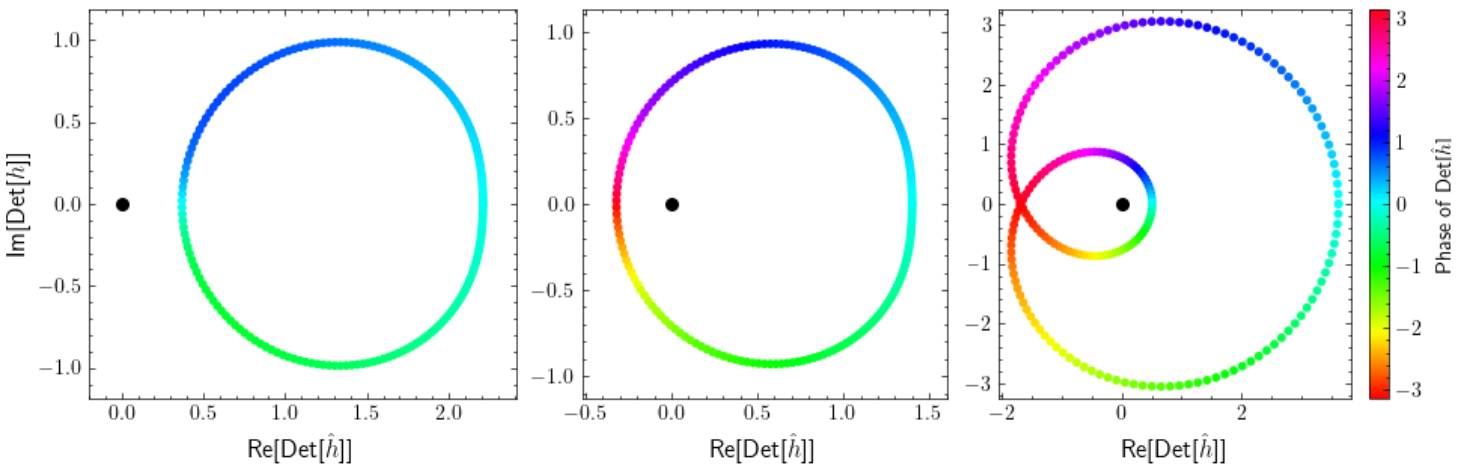
\includegraphics[width=\linewidth]{media/sp-ssh-012.png}
	\caption[Topología de la Red SP-SSH para $\Delta\beta = 0$.]{Topología de la Red SP-SSH para $\Delta\beta = 0$. Determinante de la matriz-bloque $\hat{h}$ para los cuasimomentos $-\frac{\pi}{a} \le k  < \frac{\pi}{a}$. Se aprecian exactamente tres fases topológicas distintas. \label{fig:sp-wilson}}
\end{figure}
Para obtener todo el diagrama de fase (en particular, para $\Delta \beta \neq 0$), basta con variar $\Delta \beta$ y observar cuando hay cierre de brecha en las bandas, como se observa en la Figura~\ref{fig:sp-ssh-phase-diagram}.  La red SP-SSH presenta dos mecanismos topológicos: uno debido a la hibridización SP y otro debido a la dimerización.

\begin{figure}[H]
	\centering
	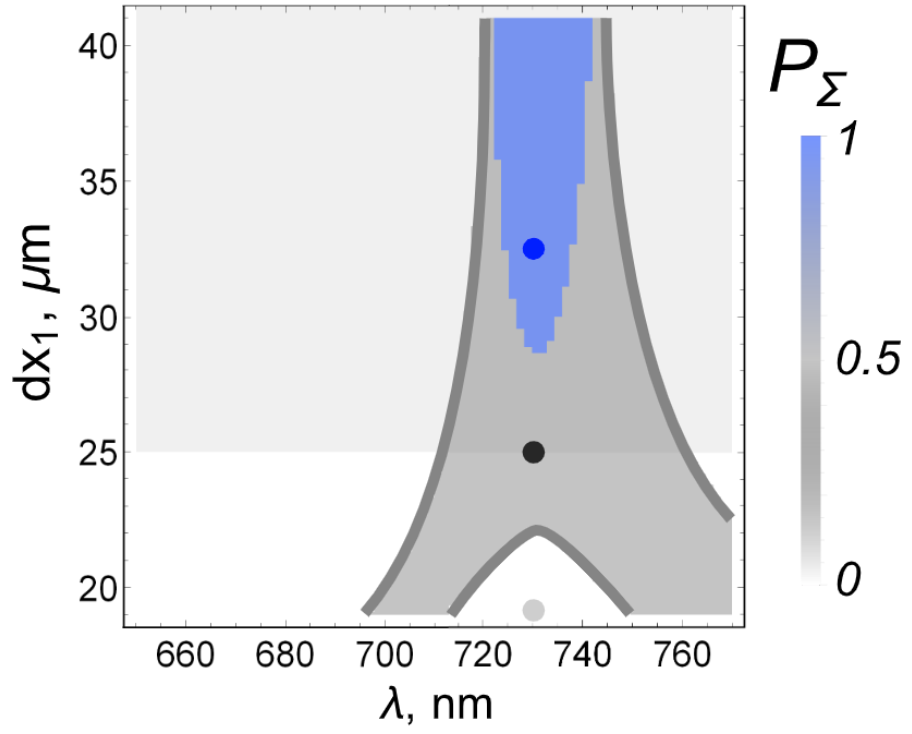
\includegraphics[width=0.4\linewidth]{media/sp-ssh-phase-diagram.png}
	\caption{Diagrama de fases topológicas. \label{fig:sp-ssh-phase-diagram}}
\end{figure}



\section{Implementación Experimental}

Para implementar experimentalmente el modelo SP-SSH, se fabricaron 25 redes fotónicas mediante la técnica de escritura con láser femtosegundo descrita en el Capítulo~\ref{cap:fs}. Los parámetros geométricos se ajustaron con separaciones entre moléculas: $dx_1$ variable, $dx_2 = 25$ $\mu$m, $dy = 20$ $\mu$m y entre guías: $dx_0 = 7$ $\mu$m. Se optimizaron los contrastes de índice de refracción para lograr degeneración de modos: $k_z^S \sim k_z^P$ en $\lambda = 730$ nm \cite{interorbital}.

Las mediciones se realizaron mediante barrido de longitud de onda (Capítulo~\ref{cap:wavelength}) con $\lambda \in$ 700 - 780 nm y paso de 5 nm. La excitación se aplicó a la guía $S$ en un extremo de la red, midiendo la potencia relativa en el mismo extremo ($I_{\text{edge}}/I_{\text{total}}$). Aunque inicialmente no se distinguen claramente las fases topológicas con polarización de bulto $P_\Sigma=1/2$ o $P_\Sigma=1$, el análisis numérico revela que durante la segunda transición topológica la razón $I_{\text{edge}}/I_{\text{total}}$ debería formar una meseta. La Figura~\ref{fig:sp-ssh-num} confirma este comportamiento, mientras que la Figura~\ref{fig:sp-ssh-exp} muestra resultados experimentales representativos: Uno para una $\lambda =$ 680 nm, donde sólo se aprecia topología por dimerización y otro para $\lambda =$ 725 nm, donde ocurre una doble transición topológica al cambiar la dimerización.

\begin{figure}[H]
	\centering
	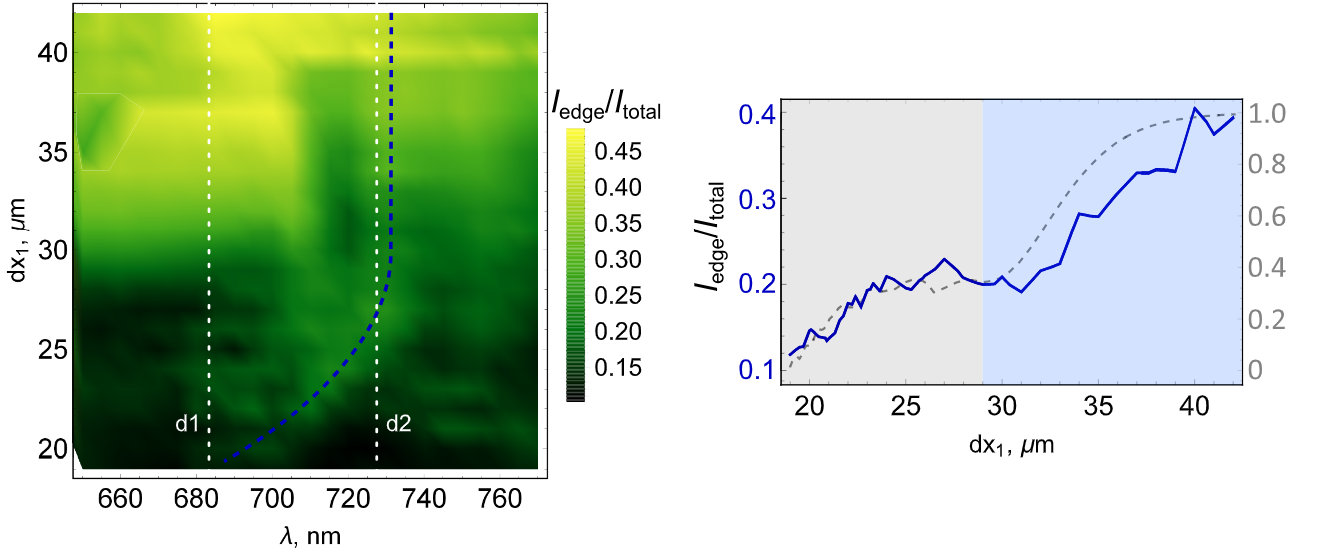
\includegraphics[width=0.9\linewidth]{media/sp-ssh-exp-num.png}
	\caption[Análisis numérico-experimental del modelo SP-SSH]{
		\textbf{Izquierda:} Resultados numéricos mostrando la meseta característica. 
		\textbf{Derecha:} Comparación cuantitativa entre datos experimentales y simulaciones.
		\label{fig:sp-ssh-num}}
\end{figure}

\begin{figure}[H]
	\centering
	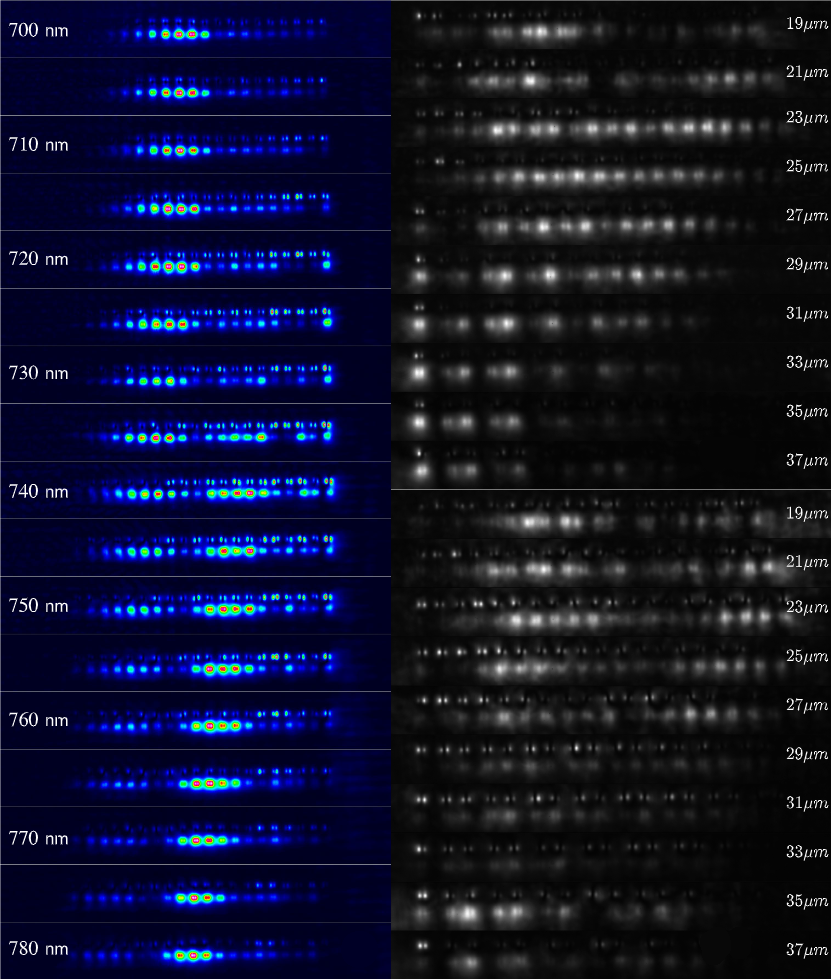
\includegraphics[width=\linewidth]{media/sp-ssh-exp.png}
	\caption[Caracterización experimental de redes SP-SSH]{
		\textbf{Izquierda:} Red SP-SSH homogénea ($dx_1 = dx_2$) para diferentes longitudes de onda. 
		\textbf{Derecha:} Arriba: Excitación en 680 nm para distintas dimerizaciones. 
		Abajo: Misma excitación en 725 nm.
		\label{fig:sp-ssh-exp}}
\end{figure}